\begin{figure}[ht]
\begin{center}
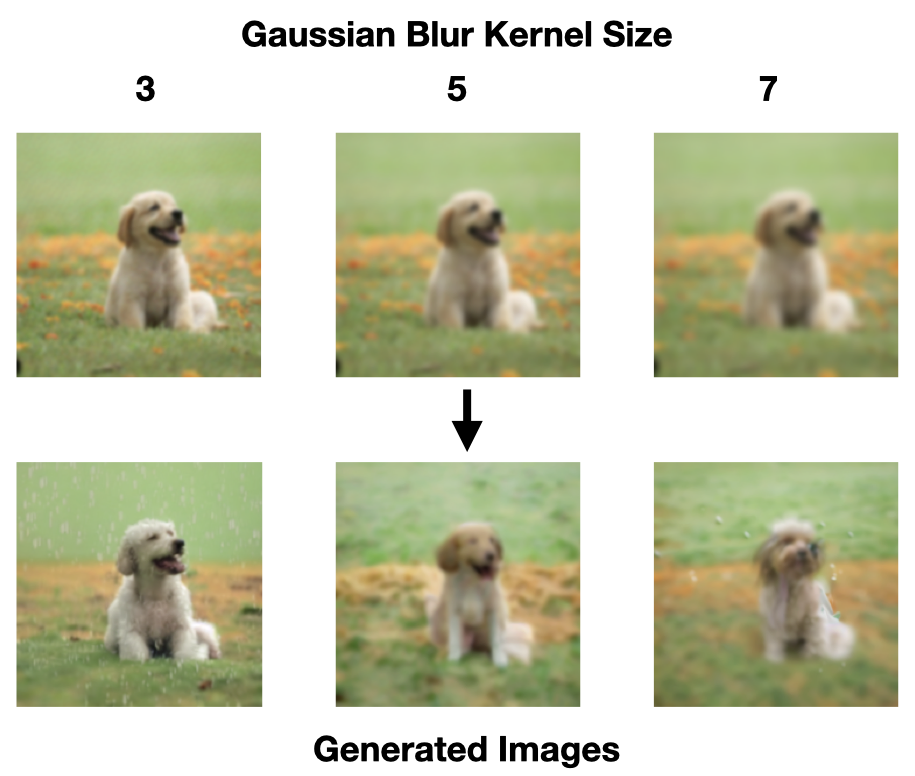
\includegraphics[width=0.55\textwidth]{images/flip-and-blur-figures.002.png}
\end{center}
\caption{\textbf{Gaussian blurs of photoguard images}. First row: We perform a Gaussian blur on a photoguard image with varying kernel sizes. Second row: Starting from the blurred image above, the adversary uses a diffusion model to make edits according to the same prompt setup as Figure~\ref{fig:img2img-overview}. With a larger kernel, the generated images lose significant visual features and do not maintain the original subject, unlike JPEG compression.}
\label{figure-gaussian-blur}
\end{figure}